\section{Auswertung}
\subsection{Temperaturverläufe}
Die Temperaturen $T_{1}$ und $T_{2}$ wurden in Grad Celsius gemessen und anschließend in Kelvin umgerechnet, was die Berechnung
der gesuchten Größen ermöglicht. Die Temperaturverläufe sind in dem folgenden Diagramm \ref{fig:plot1} dargestellt.
\begin{figure}[h]
  \centering
  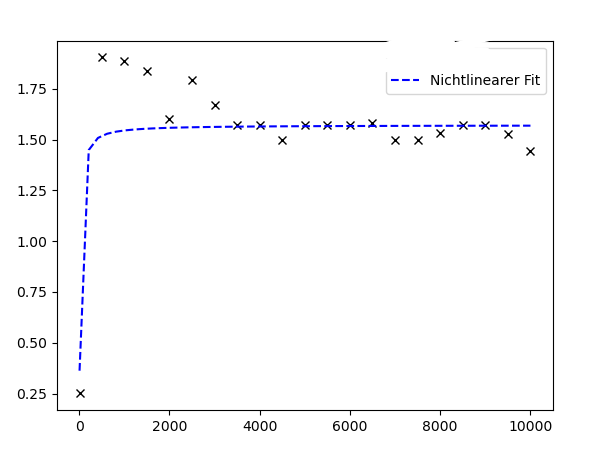
\includegraphics[width=\textwidth]{build/plot1.pdf}
  \caption{Messdaten der Temperaturen}
  \label{fig:plot1}
\end{figure}
\begin{flushleft}
Dabei wurde die Abszisse als Zeit $t$ in Sekunden gewählt. Nun lässt sich eine Ausgleichsfunktion durch
die einzelnen Messwerte legen, dafür wurde hier ein Polynomansatz zweiten Grades gewählt. Also
\end{flushleft}
\begin{equation}
T(t) = \symup{A} t^{2} + \symup{B} t + \symup{C}
\end{equation}
Die Parameter, inklusive Fehler, lassen sich beispielsweise mit einem curvefit in python berechnen.
Für die erste Ausgleichsfunktion $T_{1}$($t$) entstehen folgende Parameter
\begin{align}
\symup{A_{1}} &= (-3.22 \pm 0.04)\cdot 10^{-6} \, \si[per-mode=symbol]{\kelvin\per\second\squared}\\
\symup{B_{1}} &= (20.00 \pm 0.09) 10^{-3} \,\si[per-mode=symbol]{\kelvin\per\second}\\
\symup{C_{1}} &= (294.97 \pm 0.04) \,\si{\kelvin}
\end{align}
Analog folgen nun die Parameter der Ausgleichsfunktion $T_{2}$($t$)
\begin{align}
\symup{A_{2}} &= (9.55 \pm 2.67)\cdot 10^{-7} \, \si[per-mode=symbol]{\kelvin\per\second\squared}\\
\symup{B_{2}} &= (-11.20 \pm 0.58) 10^{-3} \,\si[per-mode=symbol]{\kelvin\per\second}\\
C_{2} &= (295.87 \pm 0.26) \,\si{\kelvin}
\end{align}
Durch das Einfügen dieser Funktionen in das Diagramm \ref{fig:plot1} kann die Plausibilität
der Parameter deutlich gemacht werden.
\begin{figure}[h]
  \centering
  \includegraphics[width=\textwidth]{build/plot2.pdf}
  \caption{Messdaten der Temperaturen und Ausgleichsfunktionen}
  \label{fig:plot2}
\end{figure}
\begin{flushleft}
Nun lassen sich jeweils vier verschiedene Messpunkte genauer betrachten und die dazugehörigen Differenzenquotienten bestimmen. Dafür wurden hier
Messstellen im Abstand von $\increment t = \SI{420}{\second}$ gewählt.
Der Differenzenquotient des Polynom zweiten Grades lautet wie folgt.
\end{flushleft}
\begin{equation}
\frac{\symup{d}T}{\symup{d}t} = 2 \symup{A} t + \symup{B}
\end{equation}
In den Gleichungen \eqref{eq25} bis \eqref{eq28} sind die ausgerechneten Differenzenquotienten des Temperaturverlaufs $T_{1}$
\begin{align}
\left( \frac{\symup{d}T_{1}}{\symup{d}t}\right)_{420} &= (17.57\pm0.1)\cdot 10^{-3} \, \text{[K/s]} \label{eq25}\\
\left(\frac{\symup{d}T_{1}}{\symup{d}t}\right)_{840} &= (14.86\pm0.12)\cdot 10^{-3} \,\text{[K/s]}\\
\left(\frac{\symup{d}T_{1}}{\symup{d}t}\right)_{1260} &= (12.15\pm0.14)\cdot 10^{-3} \, \text{[K/s]}\\
\left(\frac{\symup{d}T_{1}}{\symup{d}t}\right)_{1680} &= (9.44\pm0.17)\cdot 10^{-3} \, \text{[K/s]} \label{eq28}
\end{align}
Für den zweiten Temperaturverlauf $T_{2}$ folgt
\begin{align}
\left( \frac{\symup{d}T_{2}}{\symup{d}t}\right)_{420} &= (-10.4\pm0.6)\cdot 10^{-3} \, \text{[K/s]} \label{eq29}\\
\left(\frac{\symup{d}T_{2}}{\symup{d}t}\right)_{840} &= (-9.6\pm0.7)\cdot 10^{-3} \,\text{[K/s]}\\
\left(\frac{\symup{d}T_{2}}{\symup{d}t}\right)_{1260} &= (-8.8\pm0.9)\cdot 10^{-3} \, \text{[K/s]}\\
\left(\frac{\symup{d}T_{2}}{\symup{d}t}\right)_{1680} &= (-8.0\pm1.1)\cdot 10^{-3} \, \text{[K/s]} \label{eq32}
\end{align}
Dabei lassen sich die Fehler über die Gaußsche Fehlerfortpflanzung berechnen.
\begin{equation}
  \increment \left( \frac{\symup{d}T}{\symup{d}t}\right) = \sqrt{\left( \frac{\partial}{\partial A} \left( \frac{\symup{d}T}{\symup{d}t} \right)\right)^{2} \cdot (\increment A)^{2} + \left( \frac{\partial}{\partial B} \left( \frac{\symup{d}T}{\symup{d}t} \right)\right)^{2} \cdot (\increment B)^{2} }
  \label{eqn:gaussianmistake}
\end{equation}
\subsection{Berechnung der Güteziffer}
Anhand der ermittelten Differenzenquotienten lassen sich nun die realen Güteziffern berechnen, dazu muss lediglich in die Gleichung \eqref{eqn:gueteziffermesswerte} eingesetzt und die
gemittelte Leistung $N$ bestimmt werden.
Die gemittelte Leistung $N$ mit Fehler des Mittelwerts lautet
\begin{equation}
\overline{N_{mech}} = (120.5 \pm 0.2) \text{W}
\end{equation}
Für die idealen Güteziffern wird nun die Gleichung \eqref{eqn:idealgueteziffer} verwendet. Die Temperaturen $T_{1}$, $T_{2}$ können durch das Polynom mit der jeweiligen Zeit $t$ berechnet werden.
\begin{table}
  \centering
  \caption{Ideale und reale Güteziffern.}
  \label{tab:gueteziffernidealundreal}
  \begin{tabular}{c c c}
    \toprule
    Zeit {$t \: [\si{\second}]$} & {$\nu_\text{ideal}$} & {$\nu_\text{real}$} \\
    \midrule
    420  & 26.14 & 2.55 ± 0.015 \\
    840  & 13.70 & 2.16 ± 0.017 \\
    1260  &  9.81 & 1.76 ± 0.02 \\
    1680 &  8.31 & 1.37 ± 0.024\\
    \bottomrule
  \end{tabular}
\end{table}
Hier entsteht die Fehlerberechnung wieder durch die Gaußsche Fehlerfortpflanzung wie zuvor, diesmal mit den fehlerbehafteten Größen $N$ und ${\symup{d}T_{1}}/{\symup{d}t}$.
Damit die Wärmepumpe möglichst effizient arbeitet, dürfen sich nach der Annahme \eqref{eqn:idealzweiterhauptsatz} die Temperaturen $T_{1}$ und $T_{2}$ praktisch nicht ändern.
Das ist bei dieser realen Wärmepumpe allerdings nicht umsetzbar, denn es lässt sich nicht vollständig verhindern, dass ein wenig Wärme an die Umgebung abgegeben wird.
Die verwendeten Parameter zur Berechnung von den Güteziffern \ref{tab:gueteziffernidealundreal} stehen im Folgenden noch einmal aufgelistet.
\begin{align}
m_{w} &= m_{k} = \SI{4}{\kilo\gram} \\
c_{w} &= \SI{4158.1}{\joule\per\kilo\gram\per\kelvin}\\
c_{k}m_{k} &= \SI{750}{\joule\per\kelvin}\\
N &= (120.5 \pm 0.15) \text{W}
\end{align}
%WERTE UND FEHLER MÜSSTEN ÜBERPUÜFT WERDEN
\subsection{Massendurchsatz}
Mit der bereits aufgestellten Gleichung \eqref{eqn:eqmassendurchsatz} kann der Massendurchsatz der einzelnen Temperaturen angegeben werden.
Dafür wird allerdings die Verdampfungswärme $L$ benötigt, welche noch unbekannt ist. Diese kann allerdings durch eine Dampfdruck-Kurve gewonnen werden, indem eine Lineare Regression durchführt wird.
Zunächst müssen auf die berechneten Drücke $p_{1}$ und $p_{2}$ jeweils 1 bar addiert werden. Anschließend kann der Druck noch in Pascal umgerechnet werden. In einem Diagramm kann nun der Logarithmus des Dampfdrucks $p_{1}$ gegen die reziproke absolute Temperatur $T_{1}$ dargestellt werden \ref{fig:plot3}.
\begin{figure}[h]
  \centering
  \includegraphics[width=\textwidth]{build/plot3.pdf}
  \caption{Messwerte in einer logarithmisch-reziproken Darstellung}
  \label{fig:plot3}
\end{figure}
Für die Berechnung der Verdampfungswärme wird nun die Lineare Beziehung \eqref{eqn:linbeziehung} verwendet. Es gilt
\begin{equation}
\text{ln} p = - \frac{\symup{L}}{\symup{R}} \frac{1}{T} + const
\end{equation}
Dabei ist $R$ die allgemeine Gaskonstante. Erkennbar ist also eine lineare Beziehung zwischen dem logarithmischen Druck und der reziproken Temperatur.
Mithilfe einer Ausgleichsgerade kann somit also die Verdampfungswärme $L$ als Steigung dieser Geraden identifiziert werden.
Verwendet wird folglich der Ansatz
\begin{equation}
\text{ln} p = - \frac{\symup{A}}{\symup{R}} \left( \frac{1}{T} \right) + \symup{B} 
\end{equation}
Hier müssen also die passenden Parameter A und B gefunden werden, was durch eine lineare Regression ermöglicht werden kann.
Die Lösungen sehen folgendermaßen aus
\begin{align}
\symup{A} &= (2.05\pm0.06)\cdot 10^{4}{\si{\kelvin}} \\
\symup{B} &= (21.65\pm0.23)
\end{align}
Mit diesen Parametern lässt sich nun eine Ausgleichsgerade in das Diagramm \ref{fig:plot3} einzeichnen.
\begin{flushleft}
Die Steigung $A$ entspricht nun der Verdampfungswärme $L$, die Verdampfungswärme pro Gramm muss also für das verwendete Gas $\ce{Cl2F2C}$ (Dichlordifluormethan) speziell berechnet werden.
Die molare Masse von $\ce{Cl2F2C}$ ist
\end{flushleft}
\begin{equation}
M = \SI{120.91}{\gram\per\mol}
\end{equation}
Daraus folgt
\begin{equation}
L = \frac{\symup{A}}{M} = (1.69 \pm 0.05) \cdot 10^{5} \, \si{\joule\per\kilo\gram}
\end{equation}
Der Fehler wird wieder durch eine Fehlerfortpflanzung mit nur einem fehlerbehafteten Wert $A$ bestimmt.
Zusammen mit \eqref{eqn:massendurchsatz2} und \eqref{eqn:eqmassendurchsatz} kann nun der Massendurchsatz geschrieben werden als
\begin{equation}
\frac{\increment m}{\increment t} = (m_{w}c_{w} + m_{k}c_{k})\frac{\increment T_{2}}{\increment t} \frac{1}{L}
\end{equation}
Für die vier verschiedenen Differenzenquotienten von $T_{2}$ folgen die Massendurchsätze
\begin{align}
\left( \frac{\increment m}{\increment t} \right)_{420} &= (1.07 \pm 0.07) \si{\gram\per\second} \\
\left( \frac{\increment m}{\increment t} \right)_{840} &= (1.00 \pm 0.08) \si{\gram\per\second} \\
\left( \frac{\increment m}{\increment t} \right)_{1260}&= (0.91 \pm 0.1) \si{\gram\per\second} \\
\left( \frac{\increment m}{\increment t} \right)_{1680}&= (0.83 \pm 0.11) \si{\gram\per\second} 
\end{align}
Anschließend ist noch einmal die konkrete Berechnung des Fehlers aufgeführt.
Für $\increment \left( \frac{\increment m}{\increment t} \right) $ gilt dann
\begin{equation}
\increment \left(\frac{\increment m}{\increment t}\right) = \sqrt{\left( \frac{m_{w}c_{w} + m_{k}c_{k}}{L} \right)^{2} \cdot \left( \increment \left( \frac{\increment T_{2}}{\increment t}\right) \right)^2 +
\left( \frac{m_{w}c_{w} + m_{k}c_{k}}{L^{2}} \frac{\increment T_{2}}{\increment t}\right)^{2} \cdot (\increment L)^2}
\end{equation}
\subsection{Mechanische Kompressorleistung}
Bei der Berechnung der mechanischen Kompressorleistung zwischen einem Druckunterschied $p_{2} - p_{1}$ wird die Dichte des Transportgases (Dichlordifluormethan) $\ce{CL2F2C}$ benötigt.
Dazu eignet sich die ideale Gasgleichung
\begin{equation}
pV = n R T = \text{const}
\end{equation}
siehe \eqref{eqn:idealegasgl}. Unter Verwendung von Normalbedingung
\begin{align}
p_{0} &= 10^{5} \, \text{Pa} \\
T_{0} &= \SI{273.15}{\kelvin} \\
\rho_{0} &= \SI{5.51}{\kilo\gram\per\meter\cubic}
\end{align}
lässt sich folgende Gleichung aufstellen
\begin{align}
p_{0} \cdot \frac{m}{\rho_{0}} = nR T_{0} &\implies p_{2} \frac{m}{\rho} = nR T_{2} \\
&\implies \rho = \frac{\rho_{0}T_{0}p_{2}}{p_{0}T_{2}}
\end{align}
Dabei ist $\rho$ die Dichte des Transportmediums bei der Temperatur $T_{2}$ und dem Druck $p_{2}$, welches zur Berechnung von der Kompressorleistung benötigt wird.
Nun lässt sich mit gegeben Isentropenkoeffizient $\kappa = 1.14$ die Kompressorleistung bestimmen.
\begin{equation}
N_{mech} = \frac{1}{\kappa - 1} \left( p_{1}\sqrt[\kappa]{\frac{p_{2}}{p_{1}}} - p_{2} \right) \frac{p_{0}T_{2}}{\rho_{0}T_{0}p_{2}} \frac{\increment m}{\increment t}
\end{equation}
\begin{flushleft}
Es ergeben sich die folgenden Werte
\end{flushleft}
\begin{table}
  \centering
  \caption{Mechanische Kompressorleistung}
  \label{tab:mechkompr}
  \begin{tabular}{c c c}
    \toprule
    Zeit {$t \: [\si{\second}]$} & Temperatur $T_{2} \, [\si{\kelvin}]$ & Kompressorleistung $N_\text{mech} \, [\si{\watt}]$ \\
    \midrule
    420  & 292.35 & 10.93 ± 0.72 \\
    840  & 288.05 & 15.7 ± 1.26 \\
    1260  &  284.05 & 17.31 ± 1.9 \\
    1680 &  281.15 & 18.8 ± 2.5\\
    \bottomrule
  \end{tabular}
\end{table}
\begin{flushleft}
Der Fehler für die Kompressorleistung lässt sich wieder mit Gauß berechnen und es ergibt sich die Gleichung.
\end{flushleft}
\begin{equation}
  \increment N_{mech} = \frac{1}{\kappa - 1} \left( p_{1}\sqrt[\kappa]{\frac{p_{2}}{p_{1}}} - p_{2} \right) \frac{1}{\rho} \cdot \increment \left( \frac{\increment m}{\increment t} \right)
\end{equation}
